\documentclass[headings=optiontohead,12pt,letterpaper,oneside,spanish]{book}
\usepackage[spanish, activeacute]{babel}% Utilizamos el paquete para utilizar espa\~nol
\usepackage[utf8]{inputenc}
\usepackage[T1]{fontenc}
\usepackage{lmodern}%Esto evita los problemas derivados al hacer dvipdf con el paquete '[T1]{fontenc}'. The Debian package that includes this fonts should be installed and its name is lmodern.deb

\usepackage{graphicx}% Utilizamos el paquete para gestionar imagenes jpg
\usepackage{amsmath}
\usepackage{amssymb}%Para simbolos matematicos como el \\mathbb{R}
\usepackage{geometry}
\geometry{verbose,letterpaper,tmargin=2.5cm,bmargin=2cm,lmargin=3.5cm,rmargin=2cm}
%\pagestyle{plain}

%Para usar Times New Roman
\usepackage{times}

%%%%%%%%%%%%%%%%%%%%%% Esto es para que la cabecera no quede con todas las letras en mayusculas %%%%%
\usepackage{regexpatch}% http://ctan.org/pkg/regexpatch
\makeatletter
% \*patchcmd{<cmd>}{<search>}{<replace>}{<success>}{<failure>}
\xpatchcmd{\chaptermark}{\MakeUppercase}{}{}{}%
%\xpatchcmd{\sectionmark}{\MakeUppercase}{}{}{}%
%\xpatchcmd*{\tableofcontents}{\MakeUppercase}{}{}{}%
\makeatother
%%%%%%%%%%%%%%%%%%%%%%%%%%%%%%%%%%%%%%%%%%%%%%%%%%%%%%%%%%%%%%%%%%%%%%%%%%%%%%%%%%%%%%%%

%\setcounter{secnumdepth}{3}
%\setcounter{tocdepth}{3}
\usepackage{longtable}
\usepackage{subfigure}
\usepackage{float}
\usepackage{epsfig}
\usepackage{listings}%para escribir codigo C
\usepackage{subfigure}%para figuras una al lado de otras

\makeatletter

\usepackage{algorithm}
\usepackage{algorithmic}

% Para atenuar el corte de palabras
\sloppy 
\hyphenpenalty=10000

%Interlineado en 1.5
\usepackage{setspace}
\spacing{1.5}


%Esto es para que se coloque la palabra 'Algoritmo' en vez de 'Algorithm'
\newfloat{algorithm}{tbp}{loa}
\floatname{algorithm}{Algoritmo}




\begin{document}

%Los 2 comando de a continuacion cambian el nombre 
%"Cuadro" por "Tabla"
\renewcommand{\listtablename}{'Indice de tablas}
\renewcommand{\tablename}{Tabla}

\thispagestyle{empty}

%\begin{flushleft}
\textbf{
\small{
\hspace{-0.2cm}UNIVERSIDAD CATÓLICA DEL MAULE  \\
Facultad de Ciencias de la Ingeniería  \hfill  Profesor Guía\hspace{-0.1cm}\\
Escuela de Ingeniería Civil Informática \hfill  Nombre\_profesor\_Guía\\
}
}
\vspace{5cm}
\begin{center}
		{\bf {\normalsize TÍTULO DE LA TESIS}}\\
\vspace{1cm}
        {\bf {\normalsize NOMBRE(S) ALUMNO(S) TESISTA(S)}}\\
\vspace{1cm}
        {\normalsize Tesis  para optar al}\\
        {\normalsize Título Profesional de Ingeniero Civil Informático}
%\end{flushleft}
\vfill
\textbf{Talca, MES 20XX}
\end{center}

\newpage

\thispagestyle{empty}

\begin{center}
\textbf{
    UNIVERSIDAD CATÓLICA DEL MAULE\\
    FACULTAD DE xCIENCIAS DE LA INGENIERÍA\\
    ESCUELA DE INGENIERÍA CIVIL INFORMÁTICA\\
}
\vspace{1.5cm}

TESIS PARA OPTAR AL\\
TÍTULO PROFESIONAL DE INGENIERO CIVIL INFORMÁTICO\\

\vspace{1.2cm}

``TÍTULO DE LA TESIS''\\
NOMBRE(S) ALUMNO(S) TESISTA(S)\\

\end{center}

\vspace{0.5cm}

%\begin{tabular}{l}
    \textbf{COMISIÓN EXAMINADORA \hfill FIRMA}\hspace*{2cm}\\
%\vspace{0.5cm}

    PROFESOR GUÍA \hfill \\
    NOMBRE\_PROFESOR\_GUÍA \hfill \_\_\_\_\_\_\_\_\_\_\_\_\_\_\_\_\_\_\_\_\_\_\_ \\
%\vspace{0.5cm}

    PROFESOR COMISIÓN \hfill \\
    NOMBRE\_PROFESOR\_COMISIÓN \hfill \_\_\_\_\_\_\_\_\_\_\_\_\_\_\_\_\_\_\_\_\_\_\_ \\
%\vspace{0.5cm}

    PROFESOR COMISIÓN \hfill \\
    NOMBRE\_PROFESOR\_COMISIÓN \hfill \_\_\_\_\_\_\_\_\_\_\_\_\_\_\_\_\_\_\_\_\_\_\_ \\
%\vspace{0.8cm}

    NOTA FINAL EXAMEN DE TÍTULO\hfill \_\_\_\_\_\_\_\_\_\_\_\_\_\_\_\_\_\_\_\_\_\_\_ \\
%\end{tabular}

\vfill

\begin{center}
\textbf{TALCA, MES DE 20XX}
\end{center}




\newpage

%\thispagestyle{empty}

%%%%%    Dedicatoria (Opcional)     %%%%%%%%%%
%\vspace{5cm}
%\begin{flushright}\textbf{\Large A Persona-1 y Persona-2}\end{flushright}



%%%%    Capítulo de Agradecimiento (Opcional)   %%%%%%
%\chapter{Agradecimientos}
%TEXTO
%\begin{flushright}\emph{Autor}, Fecha.\end{flushright}



\chapter*{Sumario}

resumen trabajo.... (máximo 3 páginas)\\

A continuación algunos ejemplos de figuras, referencia, cita, tabla y algoritmo:\\

\begin{figure}
\begin{center}
   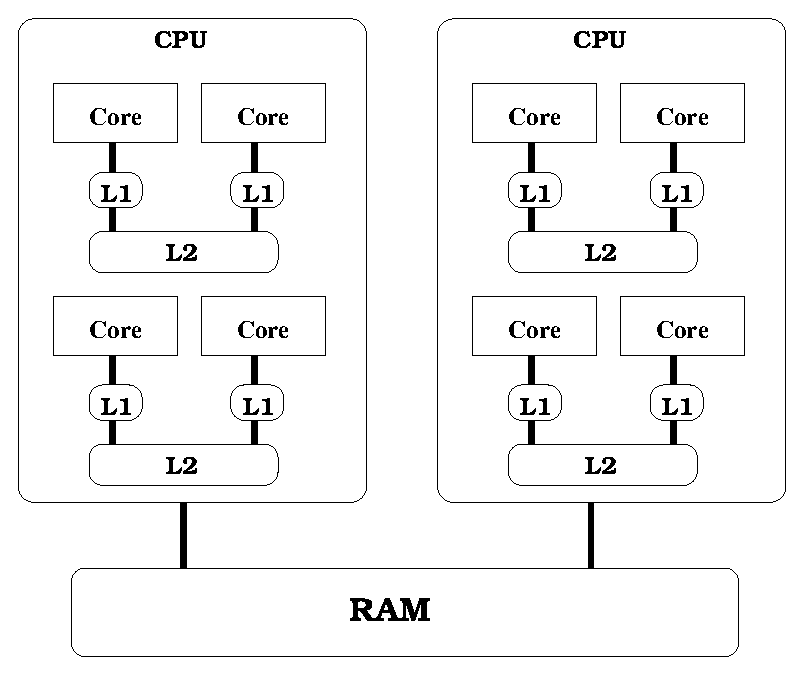
\includegraphics[scale=0.5]{fig/plataforma.eps}
\end{center}
\caption{\label{fig:plataforma}Plataforma multi-core.}
\end{figure}


Una referencia a la Figura \ref{fig:plataforma} y a las subfiguras \ref{cod_gpu_sync-a} y \ref{cod_gpu_sync-b}.
Una cita a libro de Pthreads \cite{libroPthreads}
y OpenMP (\cite{libroOpenMP}).

\begin{figure}
\begin{center}
\subfigure[Caption Subfigura 1]{
	\includegraphics[width=3.5cm,height=4cm]{fig/cod_gpu_sync-a.eps}
    \label{cod_gpu_sync-a}
}~~~~~~~~~~~~
\subfigure[Caption Subfigura 2]{
	\includegraphics[width=3.5cm]{fig/cod_gpu_sync-b.eps}
    \label{cod_gpu_sync-b}
}
\caption{\label{cod_gpu_sync}Ejemplos para ilustrar la sincronizaci'on
de los threads de un \emph{warp}.}
\end{center}
\end{figure}
%Los caracteres '~' sirven para controlar el espacio entre las figuras. Si están presentes entonces las figuras quedarán una al lado de la otra obligatoriamente.



\begin{algorithm}
busquedarango(Nodo \emph{P}, Consulta \emph{q}, Rango \emph{r})
\footnotesize{
\begin{algorithmic}[1]
\STATE \COMMENT{Sea R el conjunto resultado}
\STATE $R \leftarrow \emptyset$
\STATE $d \leftarrow dist(p_0,q)$
\IF{$d<=r$}
\STATE se reporta $p_0$
\ENDIF
\STATE $range(p_0,q)\leftarrow [d-r,d+r]$
\FORALL {$ x \in P$}
\IF{$range(p_0,q) \cap range(p_0,D_{p_x}) \neq \emptyset$}
\STATE se agrega $x$ a $R$
\IF{$dist(x,q)<=r$}
\STATE se reporta $x$
\ENDIF
\ENDIF
\ENDFOR
\FORALL {$ p_i \in R$}
\STATE busquedarango($D_{p_i}$,q,r)
\ENDFOR

\end{algorithmic}
}
\caption{\emph{\label{cap:ALGgnat:-b=FAsqueda-por-rango}EGNAT}: b'usqueda por
rango $r$ para la consulta $q$.}
\end{algorithm}


   \begin{table}
\begin{center} 
   \caption{\label{tabla_hardware} Caracter'isticas Generales}
   \begin{tabular}{|c|c|}
\hline
   Processor& 2xIntel Quad-Xeon (2.66 GHz)\\
   \hline
   L1 Cache&8x32KB + 8x32KB (inst.+data)\\
   &8-way associative, 64byte per line\\
   \hline
   L2 Unifed Cache&4x4MB (4MB shared per 2 procs)\\
   &16-way associative, 64 byte per line\\
   \hline
   Memory&16GBytes\\
   & (4x4GB) 667MHz DIMM memory\\
   & 1333 MHz system bus\\
   \hline
   Operating System&GNU Debian System Linux\\
   &kernel 2.6.22-SMP for 64 bits\\
   \hline
   \end{tabular}
\end{center}
   \end{table}



\tableofcontents{}

\listoffigures

\listoftables

\listof{algorithm}{\'Indice de Algoritmos}

\mainmatter


%%%  CAPÍTULOS  %%%

\chapter[Introducción]{\label{ch:intro}Introducción}

texto...


\section{Objetivos}

El objetivo general de esta tesis se centra en la recopilación de algoritmos de vecinos más cercanos (k-nearest neighbor) encontrados en la literatura que proponene una solución más optima en tiempos de ejecución, para esto se establecio que los objetivos que cumplen con esta condición son aquellos que han sido propuestos en las lineas de paralelismo, donde a su vez se emplean heap para la resolución de este algoritmo.

Para poder realizar la unión de los diferentes algoritmos paralelos, se propone un software el cual permite la agrupación de algoritmos de diferentes plataformas paralelas, además de añadir el algoritmo secuencial base como un agregado. En base a lo anteriormente mensionado se pretende que el software sea diseñado en consideración a usuarios los cuales no esten familiarizados con la programación de estos metodos, de modo que la utilización del software no se vea ligada a sus conocimientos en áreas de programación, además tomar en consideración que la 


Los objetivos específicos son los siguientes:

\begin{itemize}
\item Realizar la interfaz gráfica del software
	Esta se realiza en JAVA debido a su capacidad de ser interpretada tanto en Windows, Linux y OSx
\item objetivo-especifico-2
\item objetivo-especifico-N
\end{itemize}




\chapter[Estado del Arte]{\label{ch:estado-arte}Estado del Arte}

El paralelimos en computación es una técnica de programación la cual permite que varias intrucciones se puedan ejecutar similtaneamente. Se base en el principio de la división de grandes problemas en varios problemas mas pequeños, que son resueltos de forma concurrente.
\\
\section{\label{sec:des-intro}Tipos de paralelismo}
Existen diversos tipos de niveles de paralelismo que se describiran a continuación:
\subsection{Nivel de bit}
En la decada de 1970 hasta alrededor de 1986, la aceleración en la arquitectura de computadores lo logro aumentar el tamaño de una palabra, reduciendo asi el numero de instrucciones que un procesador debia realizar, de este modo se logro por ejemplo reducir el proceso de instrucciones en un procesador de 8 bits al sumar dos números de 16 bits.

\subsection{Nivel de instrucción}
Los avances en esta área se realizarón alrededor de 1980 y 1990, donde esto constaba con el reordenamiento y combinación de instrucciones en grupos que luego son ejecutadas en paralelo sin cambiar el resultado del programa. Actualmente los procesadores cuentan con "pipeline" de instrucciones de varias etapas, Cada etapa en el pipeline corresponde a una acción diferente que el procesador realiza en la instrucción correspondiente a la etapa; un procesador con un pipeline de N etapas puede tener hasta n instrucciones diferentes en diferentes etapas de finalización.
\subsection{Datos}
\subsection{Tareas}
\chapter[Marco Teórico]{\label{ch:marco-teorico}Marco Teórico}

bla bla....

\chapter[Desarrollo]{\label{ch:desarrollo}Desarrollo}

\section{\label{sec:des-intro}Introducción}

En este capitulo se describirá el proceso de creación del Software mencionado ya anteriormente en capítulos previos, en los cuales se indica que el software contiene una recopilación de diversos algoritmos K-nn en diferentes plataformas paralelas y además del K-nn secuencial para equipos que no posea las características necesarias para utilizar este software, de este modo se presentara desde la metodología utilizada hasta su desarrollo final con el software en su primera versión terminada. 
Para ello sera necesario describir procesos y etapas que se dividirían en este capitulo.

\section{Metodología}   

La metodología utilizada es el desarrollo incremental (iterativo y creciente)
\\
Defino por José Joskowicz de la siguiente manera:
\\
\textit{$"$El modelo incremental consiste en un desarrollo inicial de la arquitectura completa del sistema, seguido de sucesivos incrementos funcionales. Cada incremento tiene su propio ciclo de vida y se basa en el anterior, sin cambiar su funcionalidad ni sus interfaces. Una vez entregado un incremento, no se realizan cambios sobre el mismo, sino únicamente corrección de errores. Dado que la arquitectura completa se desarrolla en la etapa inicial, es necesario, al igual que en el modelo en cascada, conocer los requerimientos completos al comienzo del desarrollo. 
Respecto al modelo en cascada, el incremental tiene la ventaja de entregar una funcionalidad inicial en menor tiempo.$"$} \cite[pág. 6 - 7]{joskowicz2008reglas}\\



\begin{figure}[hbtp]
\centering
\includegraphics[scale=0.4]{fig/incremental.png}
\caption{\label{metodologia} Modelo incremental}
\end{figure}

En relación con la figura \ref{metodologia}, el modelo incremental aplica secuencias lineales en forma escalonada a medida que avanza el calendario de actividades. Cada secuencia lineal produce “incrementos” de software susceptibles de entregarse \cite{libromcd} de manera parecida a los incrementos producidos en un flujo de proceso evolutivo. \cite[pág. 35]{pressman1988ingenieria}\\


\textit{El desarrollo incremental es útil en particular cuando no se dispone de personal para la implementación completa del proyecto en el plazo establecido por el negocio. Los primeros incrementos se desarrollan con pocos trabajadores. Si el producto básico es bien recibido, entonces se agrega más personal (si se requiere) para que labore en el siguiente incremento. Además, los incrementos se planean para administrar riesgos técnicos. Por ejemplo, un sistema grande tal vez requiera que se disponga de hardware nuevo que se encuentre en desarrollo y cuya fecha de entrega sea incierta. En este caso, tal vez sea posible planear los primeros incrementos de forma que eviten el uso de dicho hardware, y así proporcionar una funcionalidad parcial a los usuarios finales sin un retraso importante.} \cite[pág. 36]{pressman1988ingenieria}\\

Se implemento esta metodología debido a la característica propia del software, donde una etapa del software no estaba ligada a otra, de manera que se agrego algoritmo por algoritmo a medida que su desarrollo se finalizaba correctamente y luego se añadían al software.


\subsection*{Ventajas del modelo}
El modelo iterativo y creciente presenta excelentes ventajas para ser aprovechadas en el desarrollo del software propuesto, tales como:
\begin{itemize}
\item No se debe esperar a que el desarrollo del sistema o software este completo para poder ser utilizado por usuarios. Donde el primer incremente es el más importante y da paso a que los usuarios interesados ya puedan utilizar el sistema o software.
\item Los usuarios pueden utilizar incrementos iniciales como el prototipo, esto genera una experiencia real sobre el cumplimiento de los requisitos del sistema o software.
\item Como el sistema se va probando gradualmente existe menos probabilidad de errores en la etapa final
\item Se entregan primero los requisitos principales de modo que al integrar nuevas características
\item Al ser un proceso iterativo da una mejor retroalimentación del sistema o software final   
\end{itemize}

En base a las ventajas mencionadas anteriormente y en base a la característica del software, se opto por emplear esta metodología. 
\begin{itemize}

\item Su primer incremento correspondió a la creación de la interfaz gráfica, ya que esta es la base de todo el software que se desarrollo y luego correspondió la comunicación entre la interfaz gráfica en JAVA y el algoritmo k-nn secuencial en el lenguaje de programación C. 
\end{itemize}

En base a las ventajas del modelo, el primer incremento cumple con el punto anterior de entregar los requisitos principales y luego poder integrar nuevas características.

\section{Selección de algoritmos}

La selección de algoritmos se realizo bajo la búsqueda de los algoritmos propuestos en la literatura que resuelven el algoritmo K-nn, con esto se realizo el filtro en base a los algoritmos que utilizan Heap.

\subsection*{Estructura Heap}\label{sec:heap}

En programación un heap es una estructura de datos del tipo $"$árbol$"$ con información de un conjunto ordenado de datos. De manera que es utilizada para implementar colas con prioridad. En este tipo de colas, el elemento a ser eliminado o borrado es el cual tiene la mayor o menor prioridad. A su vez en cualquier momento se pueden insertar elementos con una prioridad arbitraria. 	
\\
Existen tres tipos de heap, de acuerdo a sus características de orden
\begin{itemize}
	\item Max heap: Es un árbol en el cual el valor del nodo padre es mayor a los valores de los nodos de sus hijos (en caso de poseer algún hijo), además de ser un árbol binario completo. Imagen de referencia \ref{fig:maxheap}\begin{figure}[hbtp]
	\centering
	\includegraphics[width=5cm]{fig/Max-Heap.png}
	\caption{\label{fig:maxheap} Ejemplo de Max Heap}
\end{figure} 
	\item Min heap: Es un árbol en el cual el valor del nodo padre es menor a los valores de los nodos de sus hijos (en caso de poseer algún hijo), además de ser un árbol binario completo. Imagen de referencia \ref{fig:minheap}
\begin{figure}[hbtp]
	\centering
	\includegraphics[width=5cm]{fig/Min-heap.png}
	\caption{\label{fig:minheap} Ejemplo de Min Heap}
\end{figure} 	  
	\item Min-Max heap: Es un árbol binario, que se construye a partir de un orden min  o max de acuerdo a los valores de los nodos, el valor del nodo padre debe ser menor que el valor del nodo hijo (En caso de poseer algún hijo), si posee uno o dos hijos estos tiene un valor superior tanto al nodo padre como también a los sus correspondientes nodos hijos, este es el procedimiento secuencialmente hasta el ultimo nodo del árbol. Imagen de referencia \ref{fig:minmaxheap}
\begin{figure}[hbtp]
	\centering
	\includegraphics[width=5cm]{fig/Min-max_heap.png}
	\caption{\label{fig:minmaxheap} Ejemplo de Min Max Heap}
\end{figure} 	
\end{itemize} 

Las operaciones basicas del un heap son las siguientes:
\begin{itemize}
	\item[1] Creación de un heap vacío.\\
	Si no existe un heap se crea la estructura.
	\item[2] Inserción de un nuevo elemento en la estructura heap.\\
	Si existe un heap se inserta el elemento aplicando criterios de ordenación, de modo de respetar el orden de los tipos de heap vistos anteriormente, el árbol se ordena de manera tal que siempre cumpla con el orden binario.\\
	Si no existe un heap se crea uno y se añade como el nodo padre.
	\item[3] Eliminación del elemento más grande del heap.\\
	Si existe un heap se puede eliminar el elemento raíz (nodo padre) del heap y el heap debe respetar el orden binario de modo que se reordena el árbol y uno de sus nodos hijos debe ocupar la raíz vacía, luego de haber ocupado ese nodo se debe comparar con los hijos si otro puede ocupar el lugar de nodo padre de acuerdo a las características del tipo de heap. 
\end{itemize}

En esta tesis se han utilizado para los algoritmos el heap de tipo Max Heap, esto debido a que el algoritmo busca los K vecinos mas cercanos donde realiza el calculo exhaustivo de la distancia entre dos elementos vectorizados dentro de una base de datos con un numero variado de elementos para comparar, de modo que en un comienzo se debe ir llenado el heap de tamaño $K$, con los primeros $K$ elementos analizados, el heap realiza su organización de árbol binaria y el nodo padre siempre sera el elemento de mas distancia al elemento comparado. De esta manera si se descubre una nueva distancia mas cercana al valor del nodo padre (raíz del árbol), se procese a eliminar el valor del nodo actual y se realiza la inserción del nuevo valor y se reordena el árbol nuevamente. Con esto solo se debe comparar con el valor del nodo padre (raíz) con cada una de las distancias que se van obteniendo y no con todos los valores dentro del heap, siendo muy útil esta estructura para realizar las consultas K-nn y además de poder reducir tiempos en comparación debido a lo mencionado anteriormente de solo comparar con el valor del nodo padre (raíz del árbol). 


\section{Selección de lenguajes}

Para la selección de un lenguaje de programación óptimo para el algoritmo K-nn, se debió considerar ciertas condiciones
\\
\begin{itemize}
\item Tipo de lenguaje
\item Tiempos de ejecución de instrucciones
\item Tiempos de ejecución de estructura heap
\item Posibilidad de utilizar librerías para trabajos en paralelismo
\end{itemize}  

\subsection*{Tipo de lenguaje}
En esta área se establecen muchas diferencias en los lenguajes de programación, como se sabe un computador solo reconoce el código binario y sus instrucciones están en ordenes de 0's y 1's. \\
En base a esto existen lenguajes de programación de acuerdo a la proximidad a la arquitectura de un hardware, existiendo las siguientes categorías.

\begin{itemize}
	\item Lenguajes de bajo nivel:\\
	Estos lenguajes son totalmente dependientes de la maquina para aprovechar al máximo las características de esta, dentro de esta categoría se consideran lenguajes como:
	\subitem •	 Lenguaje de maquina 
	\subitem •	 Lenguaje ensamblador 

	\item Lenguajes de alto nivel:\\
	Estos lenguajes son los mas lejanos a la arquitectura de un computador, de modo que son totalmente independientes de la maquina y muy cercanos al lenguaje humano, dentro de esta categoría se consideran lenguajes como:
	\subitem •	 Python
	\subitem •	 Fortran
	\subitem •	 Etc
	
	\item Lenguajes de medio nivel:\\
	Estos lenguajes se encuentran en un punto medio de entre los dos anteriores, debido a que su sintaxis se asimila al lenguaje humano pero se puede acceder a registros del sistema o direcciones de memoria, estas características son de lenguajes de bajo nivel, dentro de esta categoría se consideran lenguajes como:
	\subitem •	 C	
\end{itemize}  

Además un lenguaje se puede agrupar en dos categorías de acuerdo a la naturaleza del lenguaje, estas categorías son:
\begin{itemize}
	\item Lenguaje interpretado	:\\
	Estos lenguajes se caracterizan por que sus instrucciones o su código fuente, escritos mayoritariamente en lenguajes de altos nivel, estos son traducidos por un interprete (o maquina virtual según sea el caso) a un lenguaje que sea comprensible por la maquina, instrucción por instrucción. Este proceso se repite cada vez que se ejecuta un código de este tipo.\\
	La principal ventaja es una gran independencia de la plataforma donde se ejecuta los códigos o instrucciones anteriormente mencionados.\\
	Su principal desventaja es el tiempo que necesitan para ser interpretados, generalmente son más lentos en tiempo de ejecución de un lenguaje compilado.  
	\item Lenguaje compilado:\\
	Estos lenguajes se caracterizan por que su código fuente escrito en alto nivel o medio nivel (C), es traducido por un compilador a un archivo ejecutable para una maquina en especifico, en otras palabras cada maquina debe compilar sus códigos fuentes. De manera que se pueden ejecutar las veces que sea necesario sin la necesidad de repetir el proceso de compilación.
\end{itemize}

\subsection*{Tiempos de ejecución de instrucciones}

Según \cite{speed} realizo la comparación en términos de velocidad de los lenguajes de programación, obteniendo los resultados como se aprecian en la siguiente figura \ref{speed} 

\begin{figure}[hbtp]
	\centering
	\includegraphics[width=15cm]{fig/speed.png}
	\caption{\label{speed} Gráfica de tiempo de velocidad}
\end{figure} 	

\subsection*{Tiempos de ejecución de estructuras Heap} 

Una métrica importante para seleccionar el lenguaje más acorde a las necesitas que requiere el algoritmo K-nn, recordando que el tiempo de ejecución de este es importante, según \cite{heap} realizo una comparación de tiempos en diversos lenguajes de programación, como C, C++ y Python, los resultados obtenidos se aprecian en la siguiente figura \ref{speedheap}

\begin{figure}
\begin{center}
\subfigure[Ejemplo Min Heap insert]{
	\includegraphics[width=7cm]{fig/tiempo.png}
    \label{maxheap}
}~~~~~~~~~~~~
\subfigure[Ejemplo Min Heap ExtractMin]{
	\includegraphics[width=7cm]{fig/timepo.png}
    \label{minheap}
}
\caption{\label{speedheap} Gráfica de tiempo de velocidad}
\end{center}
\end{figure}

Como se aprecia en la figura \ref{speedheap} el tiempo de ejecución de un heap es menor en C vs C++ / Python, de manera que considerando los tiempos de ejecución el lenguaje de programación C es superior en base a esta características. 

\subsection*{Posibilidad de utilizar librerías para trabajos en paralelismo}

Basado en la guía de programación en paralelo \cite{acosta2012guia}, se establecen los conceptos básicos de la programación en paralelo basado tres en diferentes modelos como son:

\begin{itemize}
	\item \textbf{MPM} - \textit{Message Passing Model} mediante la librería \textbf{MPI}
	\\\\
	Este modelo aprovecha los múltiples \textit{cores} de trabajo que están instalados en los equipos de nueva tecnología. Se asume el \textit{hardware} como reunión de diferentes procesos a través de una red de interconexión donde cada uno tiene acceso directo y exclusivo a la información almacenada en su propia memoria local.\\
	
	MPM maneja un tipo de acceso a memoria denominado \textbf{NUMA} \textit{(Nom-Uniform Memory Access)}. En el que se describe que los procesos que se comunican por la red escalable de interconexión.\\
	El hardware a su vez, cada memoria esta conectada directamente a una CPU, en vez de estar controlado a una memoria (modelo UMA). Las CPUs están conectadas con un I/O hub que permite el ordenamiento de los datos y reduciendo los problemas de tráfico.\\
	Para el uso de un programa en MPM se debe especificar el número de procesos que cuenta la aplicación, cada proceso posee un ID o Rank.\\

	Los mensajes de MPM generalmente contienen:
		\subitem •	 La variable en la que reposan los datos que se envían.
		\subitem •	 La cantidad de datos que se envían.
		\subitem •	 El proceso receptor, el que recibe el mensaje.
		\subitem •	 Los datos que se esperan recibir por parte del receptor.
		\subitem •	 El tipo de dato que se envía.
		\subitem •	 El proceso emisor del mensaje.
		\subitem •	 La ubicación o espacio en memoria (puntero en C) donde se almacenarán los datos.\\
       
	\item Librería MPI

	La primera versión de esta librería en 1993 utilizo PVM V3 \textit{(Parallel Virtual machine)}, luego en 1994 se ajustaron complementos a la librería de PVM y nace la primera versión de MPI 1.0 \textit{(Message Passing Interface)}\\
	Una característica llamativa de MPI es que permite trabajar con grupos de procesadores definidos según el programador lo disponga mediante objetos virtuales denominados comunicadores, que permiten distribuir los recursos según la tarea a realizar.
Con la librería MPI se debe tener claro que sólo se puede declarar una única vez el ambiente en paralelo (sección comprendida entre las funciones MPI\_Init y MPI\_Finalize) y que todo el código que este dentro de la zona se ejecutará en simultáneo por todos los procesos.  
\\
Dentro de los grupos de funciones para MPI se destacan algunas como:
\subitem •	 Funciones de control de flujo: permiten crear y establecer parámetros de la sección en paralelo como número de procesos a usar, el comunicador, los ID de los procesos de la aplicación, etc.
\subitem •	 Funciones para el manejo de grupos y comunicadores: facilitan la conformación de los grupos de procesadores.
\subitem •	 Funciones de administración de recurso.
\subitem •	 Funciones de comunicación: permiten la interacción (enviar y recibir información) entre diferentes procesos. Según el número de procesos presentes en la comunicación ésta se clasifica en punto a punto y multipunto.
\subitem •	 Funciones para comunicación punto a punto: implican la interacción de dos procesos exclusivamente (maestro y esclavo), que según el tipo de petición para establecer la conexión se dividen en método bloqueante y no bloqueante.
\subitem •	 Funciones para comunicación multipunto: interactúan con múltiples procesos simultáneamente, el uso de ellas requiere que el desarrollador tenga claro el recurso con el que cuenta.\\\\
	
	\item \textbf{SMM} - \textit{Shared Memory Model} mediante la librería \textbf{OpenMP} 
	\\\\
	El modelo SMM es una abstracción del modelo de multiprocesamiento centralizado. El método de acceso a memoria es llamado UMA (\textit{Uniform Memory Access}), también conocido como SMP (\textit{Symmetric Multi- Processing}).
	
El hardware en SMM está basado en FSB (front-side bus) que a su vez es el modelo acceso a memoria usado en UMA (Uniform Memory Access). Consta de un controlador de memoria (MCH) al que se conecta a la memoria general, las
CPU interactúan con el MCH cada vez que necesitan acceder a memoria. También, cuenta con un controlador de I/O que se conecta al MCH.

SMM está fundamentado en un modelo de ejecución denominado \textit{fork/join} que básicamente describe la posibilidad de pasar de una zona secuencial ejecutada por un único hilo maestro (\textit{master thread}) a una zona paralela ejecutada por varios hilos esclavos (\textit{fork}), posteriormente, cuando finalice la ejecución en paralelo, la información y resultados se agrupan de nuevo mediante un proceso de escritura en memoria en un proceso llamado \textit{join}.\\

	\item Librería OpenMP
	\\
La gran portabilidad es una característica de MPI debido a que está soportado para C, C++ y Fortran, disponible para sistemas operativos como Solaris, AIX, HP-UX, GNU/Linux, MAC OS, y Windows.\\
Además, OpenMP soporta la interacción con el modelo de paso por mensajes (MPM) permitiendo la integración de la librería MPI en las aplicaciones, lo que amplía aún más las alternativas de programación.\\
Una particularidad de OpenMP es que permite administrar el recurso en rutinas que contienen cálculos iterativos, mediante la distribución de iteraciones de los ciclos en los diferentes threads (hilos) que maneja la aplicación mediante funciones especiales denominadas constructores.
\\\\	
	
	\item \textbf{CUDA} - \textit{(Compute Unified Device Architecture)}
	
	La Gpu \textit{(Graphic Processing Unit)} se caracteriza por tener funciones de punto flotante, en sus inicios nacio como alternativas para grandes volúmenes de información, aplicables en el desarrollo de videojuegos, reproductores de video y simulaciones complejas. Posteriormente se el modelo de programación extendida a C genero lo que hoy se conoce como CUDA.\\
El hardware de CUDA se compone por la CPU de un equipo principal o host y una GPU dispuesta en un dispositivo externo o device.\\

Las ventajas de programación en GPU son:


\subitem • Código compacto: una instrucción define N operaciones.
\subitem •  Reduce la frecuencia de los saltos en el código.
\subitem • No se requiere de hardware adicional para detectar el paralelismo.
\subitem • Permite la ejecución en paralelo asumiendo N flujos de datos paralelos.
\subitem • No maneja dependencias.
\subitem • Usa patrones de acceso a memoria continua.
		
Ademas cuenta con varias memorias tales como: \textit{Memoria compartida de lecto/escritura.}- \textit{Memoria de constantes} - \textit{Memoria de texturas}   		
	
\end{itemize}   

En base a todos los puntos mencionados y dadas cada una de las características se opto por el \textit{Lenguaje de programación C} debido a ser un lenguaje de nivel medio, el que permite acceder a direcciones de memoria como un lenguaje de bajo nivel y además de su sintaxis estar considerada como alto nivel, esto lo hace un lenguaje más potente  en esta linea, también cabe destacar que el lenguaje de programación C es un lenguaje compilado, esto permite que no se necesita utilizar de una maquina virtual o un interprete para procesar sus ejecuciones o el código fuente como lo realizan otros lenguajes, con esto solo se debe compilar una vez y ejecutar el código iterativamente. En términos de tiempos de ejecución de instrucciones como se aprecia en la gráfica de la figura \ref{speed}, se aprecia que el lenguaje de programación C es más veloz que muchos otros lenguajes, debido a las características ya mencionadas.\\
Ya acotando el rango de lenguajes entre C, C++, Python como se aprecia en la gráfica \ref{speedheap}, el lenguaje de programación C es considerablemente mas veloz para procesar la estructura Heap y a esto se le añade la característica de ser un lenguaje que soporta paralelismo en todas las plataformas y cuenta con diversas librerías como se menciono anteriormente, siendo utilizadas en esta tesis OpenMP y CUDA en la cual ambas son soportadas en el lenguaje de programación C.

\section{Desarrollo interfaz}

En esta sección se aborda como se desarrolló la interfaz gráfica, en un principio se estableció \textit{JAVA} como el lenguaje de programación y se utilizo el IDE \textit{netbeans}  \cite{netbeans}, a continuación se explican cada uno de los pasos tomados en consideración al realizar la interfaz gráfica.
\\
En un principio se estableció \textit{JAVA} debido a su capacidad de ser soportado por diversos sistemas operativos, como son Windows, OSx, Linux. Dado que JAVA es un lenguaje interpretado y no compilado, el interpretador (Maquina virtual) de Java es soportado por todos los sistemas antes mencionados, además el uso de \textit{netbeans} permite la fácil creación de una interfaz gráfica, esto debido a poseer \textit{drag and drop} para sus componentes gráficos, en otras palabras solo se necesita arrastrar una componente y situarla en la posición necesaria, esta ventaja dada por \textit{netbeans} es útil, debido al menor tiempo que se ejecuta para crear la interfaz y poder otorgar el tiempo a las funciones correspondientes.\\

Otra característica importante de \textit{JAVA} se debe a que se puede realizar la ejecución de los ejecutables creados luego de la compilación de los algoritmos K-nn y retornar los valores del ejecutable a la interfaz, de esto se logra poder potencial de mejor manera el software. De modo que la interfaz gráfica solo realiza funciones de selección de bases de datos y campos de formularios, en otras palabras la interfaz gráfica solo es una fachada con la finalidad de no realizar la ejecución de los algoritmos desde la terminal.
\\\\
La figura \ref{interfaz_inicial} muestra la interfaz de usuario cuando el software inicia, la cual se compone de la barra superior la cual posee dos menús $"$File$"$ y $"$Menus$"$, una sección de \textit{input} que corresponde a los datos de entrada para el algoritmo K-nn, una sección de \textit{Result} donde en el primer recuadro de la izquierda se muestra la vista previa de las primeras 1000 lineas del archivo de base de datos, en el recuadro central se muestra la vista previa de las primeras 1000 lineas del archivo de consultas, en el cuadro de la derecha muestra los resultados del proceso, muestra si la carga de los datos fue exitosa, el tiempo de ejecución o algún error que pudiese haber ocurrido, como el fallo en la carga de los datos. En la parte inferior del software indica la cantidad de núcleos que posee la maquina donde el software esta instalado.

\begin{figure}[hbtp]
	\centering
	\includegraphics[width=14cm]{fig/interfaz1.png}
	\caption{\label{interfaz_inicial} Interfaz gráfica inicial del software}
\end{figure}      

\subsection*{Menús del software} \label{sec:menu}
El software posee dos menús como se menciono anteriormente, estos corresponden a $"File"$ y $"Menus"$, en el primer menú $File$ posee dos sub-menús $New$ y $Exit$, El primero posee sub-menús que corresponde a los algoritmos que posee el software, estos son:

\begin{itemize}
	\item \textit{Secuencial}
	\item \textit{Multihilos}
	\item \textit{Xeon Phi}
	\item \textit{GPU}
\end{itemize}

Cada uno de estos sub-menús, posee al menos un item que corresponde al algoritmo K-nn programado de acuerdo a la lógica que su nombre indica, esto quiere decir que el sub-menú Multihilos cuenta con a lo menos un item que permite ejecutar el algoritmo K-nn Multihilos, donde este utiliza \textit{OpenMP} para utilizar de mejor manera los recursos de la CPU.\\

Al seleccionar un item del sub-menú \textit{Multihilos} la interfaz gráfica tiene las siguientes características como se aprecia en la figura \ref{interfaz_multihilo}, en la sección $input$ se visualizan los campos de entrada que posee el software, en primer caso es la base de datos, esta se carga mediante el botón examinar, para cargar los datos de consulta se utiliza el botón examinar, $size obj$ es un valor numérico que corresponde a la magnitud del vector ingresado en la base de datos y base de consultas, $K$ es la cantidad de vecinos más cercanos que se desea obtener, $Threads$ por defecto se utiliza la cantidad cantidad de núcleos que posee la maquina donde esta instalado el software, este valor puede ser modificado por la cantidad de hilos que desea el usuario.\\
Además se cuenta con el botón $Start$ para comenzar a ejecutar el las consultas K-nn, se añadió bajo el botón $Start$ un \textit{check box} que permite ejecutar un $Profiler$ que utiliza la librería PapiC \cite{iclit2017} que indica estadísticas sobre el uso de los hilos. En la sección $Result$ no varia en relación al item seleccionado.
 
\begin{figure}[hbtp]
	\centering
	\includegraphics[width=14cm]{fig/interfaz_multicore}
	\caption{\label{interfaz_multihilo} Interfaz gráfica item multihilos del software}
\end{figure}
     
Al seleccionar un item del sub-menú \textit{Secuencial} la interfaz gráfica tiene las siguientes características como se aprecia en la figura \ref{interfaz_secuencial}, en la sección $input$ se visualizan los campos de entrada que posee el software, en primer caso es la base de datos, esta se carga mediante el botón examinar, para cargar los datos de consulta se utiliza el botón examinar, $size obj$ es un valor numérico que corresponde a la magnitud del vector ingresado en la base de datos y base de consultas, $K$ es la cantidad de vecinos más cercanos que se desea obtener.\\

\begin{figure}[hbtp]
	\centering
	\includegraphics[width=14cm]{fig/interfaz_secuencial}
	\caption{\label{interfaz_secuencial} Interfaz gráfica item secuencial del software}
\end{figure}
 
La selección de los otros item en los sub-menús son similares a los antes mencionados, de modo que solo varia la cantidad de datos de entrada que se ingresan dado las condiciones de programación de cada algoritmo.
\\\\
Además el software cuenta con mensajes dirigidos al usuario, estos son dividen en mensajes de alerta y mensajes de éxito. El primero se aprecia en la figura \ref{mensajes}\subref{fig:error}, este mensaje aparece una vez que se presiona el botón $Start$ y si algún campo esta vacío, indica que campos debe completar para poder ejecutar correctamente el proceso. Si no presenta errores el proceso parte correctamente, si los archivos de bases de datos y consultas son archivos correspondientes, el proceso muestra un mensaje de éxito, como se aprecia en la figura \ref{mensajes}\subref{fig:exito}, al presionar el botón aceptar se muestra la ventana de los resultados de la consulta K-nn, este paso corresponde a la sección \ref{sec:resultados} \textit{Métodos de exportación de resultados}.  

\begin{figure}
\begin{center}
\caption{\label{mensajes} Mensajes al usuario }
\subfigure[Mensaje 1 - Error]{
	\includegraphics[width=5cm]{fig/error}
    \label{fig:error}
}~~~~~~~~~~~~
\subfigure[Mensaje 2 - Éxito]{
	\includegraphics[width=5cm]{fig/exito_knn}
    \label{fig:exito}
}
\end{center}
\end{figure}

\section{Integración de algoritmo K-nn Secuencial} \label{met:secuencial}

Si bien este algoritmo, no estaba considera en un comienzo este se añadió para la posibilidad de poder ejecutar el software en equipos que no cuenten con procesadores con multi-núcleos y necesiten realizar consultas K-nn. Este algoritmo se realizado con la estructura heap \ref{sec:heap}.\\
Para implementar el algoritmo K-nn secuencial, se definió la estructura heap, la cual se aprecia en el segmento de código en el algoritmo \ref{lst:heap}, este almacena en $doble$ $dist$, la distancia del elemento consultado esta es de tipo $double$ debido a que las distancias son reales y puede ser el caso que se necesite almacenar un valor muy grande, a su ves $int ind$ indica la posición del vector dentro de la base de consultas. Cabe recalcar que solo se almacenan K resultados en esta estructura, además de solo almacenar los valores cuya distancia $dist$ sean las k menores.
\\ 
\begin{algorithm}
\begin{lstlisting}[language=C] 
struct _Elem {
    double dist;
    int ind;
};
typedef struct _Elem Elem;
\end{lstlisting}
\caption{\emph{\label{lst:heap}} Estructura para realizar los $Heap$.}
\end{algorithm}

Con el lenguaje de programación C, es posible utilizar la cantidad de memoria justa gracias a la instrucción $malloc$ que permite asignar la cantidad de memoria que corresponde al tamaño de la base de datos y la base de consulta, tal como se aprecia en el algoritmo \ref{lst:malloc}. Donde $consultas$ se crea una matriz de $N\_queries x DIM$ donde $N\_queries$ es el número tuplas de vectores contenidas en la base de consulta y $DIM$ es el tamaño del vector. De manera análoga se establece la matriz $DB$ de $N\_DB x DIM$ donde $N\_DB$ es el número tuplas de vectores contenidas en la base de datos y $DIM$ es el tamaño del vector. A su vez $answer$ corresponde a la asignación de memoria para las $N\_queries$ con $K$ vecinos más cercanos donde se almacenan todas las respuestas a las consultas para ser finalmente mostrados. $Heap$ es la estructura a utilizar con cada consulta, esta corresponde a un heap del tipo heap max, donde el nodo padre es el mayor valor de la estructura.
\\
El desarrollo central del algoritmo para obtener los k vecinos más cercanos esta dado por el algoritmo \ref{lst:knn}, este algoritmo indica las siguientes acciones, se establece un contador $n\_elem$ $=0$ que obtiene el número de elementos que han ingresado al heap, este se utiliza como comparador debido a que se deben ingresar k elementos al heap, mientras $n\_elem$ sea menor que el número $k$ se ingresaran los datos al heap en caso contrario se compara si la distancia del elemento actual es menor a la raíz del heap de manera que si el elemento es menor se extrae la raíz y se añade el elemento actual y se reordena el heap. Este proceso itera exhaustivamente hasta que no queden elementos en la base de datos, cuando el heap esta finalizado se almacenan sus resultados en la matriz $answer$ y se debe continuar con la siguiente consulta hasta que se realicen todas las consultas del base de consultas.

\begin{algorithm}
\begin{lstlisting}[language=C]
    Consultas = (double **) malloc(sizeof (double *)*N_QUERIES);
    for (i = 0; i < N_QUERIES; i++)
        Consultas[i] = (double *) malloc(sizeof (double)*DIM);

    DB = (double **) malloc(sizeof (double *)*N_DB);
    for (i = 0; i < N_DB; i++)
        DB[i] = (double *) malloc(sizeof (double)*DIM);

    answer = (Elem *)malloc(sizeof(Elem)*N_QUERIES*TOPK);
    
    heap = (Elem *) malloc(sizeof (Elem) * TOPK);
\end{lstlisting}
\caption{\emph{\label{lst:malloc}} Utilización de $malloc$.}
\end{algorithm}


\begin{algorithm}
\begin{lstlisting}[language=C]
for (i = 0; i < N_QUERIES; i++) {
	n_elem = 0;
	for (j = 0; j < N_DB; j++) {    
		d = distancia(Consultas[i], DB[j]);
		if(n_elem<TOPK){
			e_temp.dist = d;
			e_temp.ind = j;
			inserta2(heap, &e_temp, &n_elem);
		}
		else{
			if (d < topH(heap, &n_elem)) {
				e_temp.dist = d;
             	e_temp.ind = j;
				popush2(heap, &n_elem, &e_temp);
		}}
	}
        for (int k = 0; k < TOPK; ++k){
        	extrae2(heap, &n_elem, &e_temp);
        	answer[i*TOPK+k].ind = e_temp.ind;
        	answer[i*TOPK+k].dist = e_temp.dist;
        }
}
\end{lstlisting}
\caption{\emph{\label{lst:knn}} Proceso iterativo de una consulta K-nn.}
\end{algorithm}

\subsection{Funciones claves del algoritmo secuencial}  \label{met:claves}

$Distancia:$ Algoritmo \ref{lst:distancia} es la función de cálculo de la distancia entre vectores, tanto del vector de la base de datos y el vector de la base de consultas, este cálculo se realiza con la formula \eqref{ecu:distancia}.\\
Dados $A$ = $(X_1,Y_1)$ y $B$ = $(X_2,Y_2)$

\begin{equation}\label{ecu:distancia}
 distancia = \sqrt{(X_2-X_1)^{2}+(Y_2-Y_1)^{2}}
\end{equation}

Esta ecuación puede ser llevada a vectores de tamaño $n$.

\begin{algorithm}
\begin{lstlisting}[language=C]
double distancia(double *p1, double *p2) {
    int i = 0;
    double suma = 0;

    for (i = 0; i < DIM; i++)
        suma += ((p1[i] - p2[i])*(p1[i] - p2[i]));
    return sqrt(suma);
}  
\end{lstlisting}
\caption{\emph{\label{lst:distancia}} Cálculo de distancias entre vectores.}
\end{algorithm}


Sumado a esta función existen las funciones para manipular un heap, estas corresponden a obtener el valor nodo padre (Algoritmo \ref{lst:top}), realizar una inserción de un elemento, extraer un elemento y una añadida para facilitar el procedimiento del algoritmo como es el caso de una extracción e inserción que se utiliza cuando se debe cambiar un nodo dentro del heap y realizar el reordenamiento del heap.
\\
El algoritmo \ref{lst:top} retorna el valor de la raíz (nodo padre) del heap si no esta vacío, en caso contrario retorna el valor maximo de un $double$.
   
\begin{algorithm}
\begin{lstlisting}[language=C]
double topH(Elem *heap, int *n_elem) {
    if (*n_elem == 0)
        return DBL_MAX;
    return heap[0].dist;
}
\end{lstlisting}
\caption{\emph{\label{lst:top}} Valor de la raíz del heap.}
\end{algorithm}

El algoritmo \ref{lst:inserta2} realiza la inserción de un elemento, guardando la distancia y la posición del elemento, el contador $n\_elem$ incrementa en 1 luego de la inserción, y se realiza el ordenamiento del heap. Esta función es la que se utiliza en el algoritmo \ref{lst:heap} hasta llenar el heap.

\begin{algorithm}
\begin{lstlisting}[language=C]
void inserta2(Elem *heap, Elem *elem, int *n_elem) {
    int i;
    Elem temp;

    heap[*n_elem].dist = elem->dist;
    heap[*n_elem].ind = elem->ind;
    (*n_elem)++;
    for (i = *n_elem; i > 1 && heap[i - 1].dist > heap[(i / 2) - 1].dist; i = i / 2) {
        temp = heap[i - 1];
        heap[i - 1] = heap[(i / 2) - 1];
        heap[(i / 2) - 1] = temp;
    }
}
\end{lstlisting}
\caption{\emph{\label{lst:inserta2}} Realiza la inserción de un elemento al heap.}
\end{algorithm}

El algoritmo \ref{lst:extrae2} realiza la extracción de un elemento, guardando la distancia y la posición del elemento, el contador $n\_elem$ decrementando en 1 luego de la extracción, y se realiza el ordenamiento del heap. Esta función es la que se utiliza para completar la matriz $answer$.

\begin{algorithm}
\begin{lstlisting}[language=C]
void extrae2(Elem *heap, int *n_elem, Elem *elem_extraido) {
    int i, k;
    Elem temp;

    (*elem_extraido).dist = heap[0].dist;
    (*elem_extraido).ind = heap[0].ind;

    heap[0] = heap[(*n_elem) - 1]; // Movemos el ultimo a la raiz y achicamos el heap
    (*n_elem)--;
    i = 1;
    while (2 * i <= *n_elem) // mientras tenga algun hijo
    {
        k = 2 * i; //el hijo izquierdo
        if (k + 1 <= *n_elem && heap[(k + 1) - 1].dist > heap[k - 1].dist)
            k = k + 1; //el hijo derecho es el mayor
        if (heap[i - 1].dist > heap[k - 1].dist)
            break; //es mayor que ambos hijos

        temp = heap[i - 1];
        heap[i - 1] = heap[k - 1];
        heap[k - 1] = temp;
        i = k; //lo intercambiamos con el mayor hijo
    }
    return;
}
\end{lstlisting}
\caption{\emph{\label{lst:extrae2}} Realiza la extracción de un elemento al heap.}
\end{algorithm}

El algoritmo \ref{lst:popush2} realiza la extracción del elemento raíz y la posterior inserción del elemento cuya distancia era menor que la distancia del elemento raíz, esta función guarda la distancia y la posición del elemento, con esto luego se realiza el ordenamiento del heap. Esta función es la que se utiliza en el algoritmo \ref{lst:heap}  cuando el heap esta lleno y se obtiene un elemento cuya distancia es menor a la distancia de la raíz.


\begin{algorithm}
\begin{lstlisting}[language=C]

void popush2(Elem *heap, int *n_elem, Elem *elem) {
    int i, k;
    Elem temp;

    heap[0].dist = elem->dist;
    heap[0].ind = elem->ind;

    i = 1;
    while (2 * i <= *n_elem) // mientras tenga algun hijo
    {
        k = 2 * i; //el hijo izquierdo
        if (k + 1 <= *n_elem && heap[(k + 1) - 1].dist > heap[k - 1].dist)
            k = k + 1; //el hijo derecho es el mayor
        if (heap[i - 1].dist > heap[k - 1].dist)
            break; //es mayor que ambos hijos

        temp = heap[i - 1];
        heap[i - 1] = heap[k - 1];
        heap[k - 1] = temp;
        i = k; //lo intercambiamos con el mayor hijo
    }
    return;
}

\end{lstlisting}
\caption{\emph{\label{lst:popush2}} Realiza la extracción y la inserción de un elemento al heap.}
\end{algorithm}

Para realizar la integración de este algoritmo en la interfaz gráfica se realizó mediante una rutina de $Java$ con $java.lang.Runtime.exec()$. La implementación de esta rutina permite ejecutar otro programa o ejecutable y obtener los resultados para ser visualizados a través de la interfaz gráfica creada en $Java$. El algoritmo \ref{lst:javarun} muestra un ejemplo simple de ejecutar un programa o ejecutable desde $Java$.

\begin{algorithm}
\begin{lstlisting}[language=Java]

import java.io.*;
 
public class llamarruntime
{
   public static void main(String[] args)
   {
      try{
         Process theProcess =
                 Runtime.getRuntime().exec(Ejecutable);
      }
      catch(IOException e){
         System.err.println("Error en el metodo exec()");
         e.printStackTrace();
      }
   } 
}
\end{lstlisting}
\caption{\emph{\label{lst:javarun}} Ejecutar un programa o ejecutable desde $Java$.}
\end{algorithm}


\section{Integración de algoritmo K-nn Paralelo Multi-hilos}


Este algoritmo a posee ciertas semejanzas y diferencias con respecto a la versión secuencial, este utiliza $malloc$ como se indica en el algoritmo \ref{lst:malloc}, estableciendo los mismos atributos y designando la memoria de la misma manera que la versión secuencial, léase \ref{met:secuencial}.
\\

A través de la librería \textit{OpenMP} establece variables de tipo compartida \textit{Shared} y variables del tipo privadas \textit{Private}, donde con una variable del tipo compartida se puede obtener su valor o realizar alguna modificación sin restricciones desde cualquier hilo, a su vez una variable del tipo privada solo puede ser accesible por un hilo y se crea una copia de la variable para tantos hilos creados existan. De esta manera se han establecido variables solo variables del tipo \textit{Shared} para este algoritmo.

El desarrollo central del algoritmo para obtener los k vecinos más cercanos esta dado por el algoritmo \ref{lst:knn2}, este algoritmo indica las siguientes acciones, se establece un contador $n\_elem$ $=0$ que obtiene el número de elementos que han ingresado al heap, este se utiliza como comparador debido a que se deben ingresar k elementos al heap, mientras $n\_elem$ sea menor que el número $k$ se ingresaran los datos al heap en caso contrario se compara si la distancia del elemento actual es menor a la raíz del heap de manera que si el elemento es menor se extrae la raíz y se añade el elemento actual y se reordena el heap. Este proceso itera paralelamente hasta que no queden elementos en la base de datos, cuando el heap esta finalizado se almacenan sus resultados en la matriz $answer$ y se debe continuar con la siguiente consulta hasta que se realicen todas las consultas del base de consultas.

\begin{algorithm}
\begin{lstlisting}[language=C]
#pragma omp master
for (i = tid; i < N_QUERIES; i += procs) {           
	n_elem = 0;
    for (j = 0; j < N_DB; j++) {           
    	d = distancia(Consultas[i], DB[j]);               
        if(n_elem<TOPK){
        	e_temp.dist = d;
        	e_temp.ind = j;
        	inserta2(heap, &e_temp, &n_elem);
        }
        else{
        	if (d < topH(heap, &n_elem)) {
            	e_temp.dist = d;
            	e_temp.ind = j;
            }}
        }
        for (j = 0; j < TOPK ; j++) {
        	extrae2(heap, &n_elem, &e_temp);
        	answer[i*TOPK+j].ind = e_temp.ind;
        	answer[i*TOPK+j].dist = e_temp.dist;
       	}
}

#pragma omp barrier
\end{lstlisting}
\caption{\emph{\label{lst:knn2}} Proceso iterativo de una consulta K-nn multi-core.}
\end{algorithm}

A diferencia del método secuencial, el método multi-paralelo utiliza la librería OpenMP, por tanto como se muestra en el algoritmo \ref{lst:knn2} \textit{\#pragma omp master} indica el trabajo en la zona paralela, de manera que el ciclo $for$ realiza un paso cíclico con una cantidad determinada de hilos dada por $procs$, donde $tid$ es el identificador de cada hilo, esto quiere que decir que si utilizo 2 hilos el hilo 0 con $tid=0$ realiza la consulta 0 y el hilo 1 con $tid=1$ realiza la consulta 1 simultáneamente finalizado el trabajo de al menos uno de estos, el hilo con su actividad finalizada toma el valor correspondiente, en caso del hilo 0 con $tid=0$ le corresponde tomar la consulta 2 y al hilo 1 con $tid=1$ le corresponde el hilo 3. Este proceso se realiza hasta llegar al final de la base de consultas $N\_queries$.\\

\subsection{Funciones claves del algoritmo multi-hilos}  

Estas funciones son las mismas que el método secuencial, donde se consideran $topH$ para saber el valor del del nodo raíz, $inserta2$ para insertar un nodo en un heap con el número de elementos menor al de k elementos, $extrae2$ extrae el nodo raíz del heap, $popush2$ realiza la extracción del nodo raíz e inserción de un nuevo nodo de menor valor que la raíz extraída, léase \ref{met:claves}
\\
Para realizar la integración de este algoritmo en la interfaz gráfica se realizó mediante una rutina de $Java$ con $java.lang.Runtime.exec()$. La implementación de esta rutina permite ejecutar otro programa o ejecutable y obtener los resultados para ser visualizados a través de la interfaz gráfica creada en $Java$. El algoritmo \ref{lst:javarun} muestra un ejemplo simple de ejecutar un programa o ejecutable desde $Java$.
 

\section{Integración de algoritmo K-nn Paralelo Xeon Phi}

A diferencia de los métodos anteriores acá se utiliza un coprocesador, de modo que se debe realizar la comunicación entre la CPU y el Coprocesador (\textit{Intel Xeon Phi}). A continuación se describe en detalle las funciones de este método.\\

Con el lenguaje de programación C, es posible utilizar la cantidad de memoria justa gracias a la instrucción $malloc$ que permite asignar la cantidad de memoria que corresponde al tamaño de la base de datos y la base de consulta, tal como se aprecia en el algoritmo \ref{lst:mallocxeon}. Donde $queries$ se crea una matriz de $num\_queries x dimaux$ donde $num\_queries$ es el número tuplas de vectores contenidas en la base de consulta y $dimaux$ es el tamaño del vector. De manera análoga se establece la matriz $db$ de $num\_db x dimaux$ donde $num\_db$ es el número tuplas de vectores contenidas en la base de datos y $dimaux$ es el tamaño del vector. A su vez $answer$ corresponde a la asignación de memoria para las $num\_queries$ con $K$ vecinos más cercanos donde se almacenan todas las respuestas a las consultas para ser finalmente mostrados. $Heap$ es la estructura a utilizar con cada consulta, esta corresponde a un heap del tipo heap max, donde el nodo padre es el mayor valor de la estructura. La Xeon phi permite solo permite realizar el trabajo con vectores de modo que las matrices deben ser trabajadas como vectores y además los vectores deben ser múltiplos de 16, de modo que para solucionar este problema y poder trabajar con la medida de cualquier vector de entrada se parametriza a su vector multiplo de 16 superior, en otras palabras si ingresa un vector de tamaño 8 se parametriza a 16, si ingresa un vector 17 se parametriza a 32 y los valores restantes son establecidos como 0, para no interferir en el cálculo de la distancia.  
\\
El desarrollo central del algoritmo para obtener los k vecinos más cercanos esta dado por el algoritmo \ref{lst:knnxeon}, este algoritmo indica las siguientes acciones, las operaciones de este algoritmo están dentro de la región paralela de la \textit{Xeon phi} (\textit{\#pragma}) de manera que se deben enviar desde la CPU a la \textit{Xeon phi} todas las variables o constantes a utilizar, donde se deben cumplir ciertas restricciones como vectorizar la matriz (explicado anteriormente), además se especifican claramente cuales son datos exclusivamente de entrada \textit{In} y exclusivamente datos de salida \textit{Out} o datos que pueden ser de entrada y salida \textit{(Inout)}. La \textit{Xeon phi} a través de la librería \textit{OpenMP} utiliza además variables de tipo compartida \textit{Shared} y variables del tipo privadas \textit{Private}, donde una variable del tipo compartida puede obtener su valor o realizar alguna modificación sin restricciones, a su vez una variable del tipo privada solo puede ser accesible por un hilo y se crea una copia de la variable para tantos hilos creados existan. A diferencia del método anterior que solo utilizaba variables tipo \textit{Shared}, en este método las variables del tipo \textit{Private} se han establecido las siguientes variables \textit{i, j, thread\_num} de modo que cada hilo puede realizar independientemente sus iteraciones en los ciclos sin ser interrumpido por otro, esto debido a que se utilizan vectores y se debe emular la lectura de la matriz a través de los vectores. Dentro de la región paralela \textit{\#pragma omp parallel} se crea un heap de tamaño \textit{K}. luego se establece un contador $n\_elem$ $=0$ que obtiene el número de elementos que han ingresado al heap, este se utiliza como comparador debido a que se deben ingresar k elementos al heap, mientras $n\_elem$ sea menor que el número $k$ se ingresaran los datos al heap en caso contrario se compara si la distancia del elemento actual es menor a la raíz del heap de manera que si el elemento es menor se extrae la raíz y se añade el elemento actual y se reordena el heap. Este proceso itera paralelamente hasta que no queden elementos en la base de datos, cuando el heap esta finalizado se almacenan sus resultados en la matriz $answer$. Este proceso dentro de la región paralela \textit{\#pragma omp parallel} realiza cada uno de los pasos mencionados por cada hilo utilizado en el proceso\\



 \begin{algorithm}
\begin{lstlisting}[language=C]
   db= (double **)malloc(sizeof(double *)*num_db);
   for (i=0; i<num_db; i++)
      db[i] = (double *)malloc(sizeof(double)*dimaux);
   queries = (double **)malloc(sizeof(double *)*num_queries);
   for (i=0; i<num_queries; i++)
      queries[i] = (double *)malloc(sizeof(double)*dimaux);
   answer = (Elem *)malloc(sizeof(Elem)*num_queries*k);

   //Se transfieren datos de una matriz a un vector
   db_vector = (double *)_mm_malloc(sizeof(double)*dimaux*num_db, 64);
   for (i=0; i < dimaux*num_db; i++)
       db_vector[i] = 0.0;
   if (sizeof(double)*dimaux*num_queries < 64)
   {
        queries_vector = (double *)_mm_malloc(sizeof(double)*16, 64);
        for (i=0; i < 16; i++)
            queries_vector[i] = 0.0;
   }
   else
   {
        queries_vector = (double *)_mm_malloc(sizeof(double)*dimaux*num_queries, 64);
        for (i=0; i < dimaux*num_queries; i++)
            queries_vector[i] = 0.0;
   }
\end{lstlisting}
\caption{\emph{\label{lst:mallocxeon}}  Utilización de $malloc$.}
\end{algorithm}

 \begin{algorithm}
\begin{lstlisting}[language=C]
   #pragma offload target(mic:0) in(dim) in(db_vector:length(num_db*dimaux)) in(queries_vector:length(num_queries*dimaux)) out(answer:length(k*num_queries))
   {
      #pragma omp parallel private(i, j, thread_num) shared(db_vector, num_db, queries_vector, num_queries, dimaux, k, answer, num_threads)
      {
         
         Elem *heap;
         heap = (Elem *)malloc(sizeof(Elem)*k);
         #pragma omp master
         {
            num_threads = omp_get_num_threads();
            printf("run with %d threads\n", num_threads);
         }
         #pragma omp barrier
         thread_num = omp_get_thread_num();
         int n_elem;
         Elem e_temp;
         double d;

         
         for(i=thread_num*dimaux; i<num_queries*dimaux; i+=num_threads*dimaux){
            n_elem = 0;
            for(j=0; j<k; j++){
               e_temp.dist = distancia(&(queries_vector[i]), &(db_vector[j*dimaux]), dimaux);
               e_temp.ind = j;
               inserta2(heap, &e_temp, &n_elem);
            }

            for(j=k; j<num_db; j++){
               d = distancia(&(queries_vector[i]), &(db_vector[j*dimaux]), dimaux);
               if(d < topH(heap, &n_elem))
                  {
                     e_temp.dist = d;
                     e_temp.ind = j;
                     popush2(heap, &n_elem, &e_temp);
                  }
            }

            for(j=0; j<k; j++){
               extrae2(heap, &n_elem, &e_temp);
               printf("%d ind = %d :: dist = %f posicion:: %d \n", j, e_temp.ind, e_temp.dist,(i/dimaux)*k+j);
               answer[(i/dimaux)*k+j].ind = e_temp.ind;
               answer[(i/dimaux)*k+j].dist = e_temp.dist;
            }


         }
         free(heap);
      }
   }   
\end{lstlisting}
\caption{\emph{\label{lst:knnxeon}} Proceso iterativo de una consulta K-nn Xeon phi.}
\end{algorithm}


\subsection{Funciones claves del algoritmo Xeon phi}

A diferencia de los métodos anteriores donde solo se utiliza una \textit{CPU}, aca se emplea tanto la \textit{CPU} como un \textit{Coprocesador} el cual solo realiza tareas especificas (léase \ref{cap:coprocesadores}). A continuación se detallan las principales funciones que se implementaron en \textit{Xeon phi}.\\ 

$Distancia:$ Algoritmo \ref{lst:distanciaxeon} es la función de cálculo de la distancia entre vectores, tanto del vector de la base de datos y el vector de la base de consultas, este cálculo se realiza con la formula \eqref{ecu:distancia}. Esta función se realiza en la \textit{Xeon phi} para indicar que se realizara en el coprocesador se utiliza la sintaxis \textit{\textbf{\_\_atribute\_\_((target(mic)))}}. Las sintaxis \textit{\textbf{\_\_assume\_aligned(), \#pragma vector aligned, \#pragma ivdep, \#pragma simd }} alinea los vectores y permite que el cálculo de la distancia se realice correctamente.
  
\begin{algorithm}
\begin{lstlisting}[language=C]
__attribute__((target(mic))) double distancia(double *p1, double *p2, int DIM){
    int i=0;
    double suma=0.0;
   __assume_aligned(p1, 64);
   __assume_aligned(p2, 64);   
    #pragma vector aligned
    #pragma ivdep
    #pragma simd
    for (i=0; i < DIM; i++){
        suma += (p1[i]-p2[i])*(p1[i]-p2[i]);
    }
    return sqrt(suma);
}
\end{lstlisting}
\caption{\emph{\label{lst:distanciaxeon}} Función distancia \textit{Xeon phi}.}
\end{algorithm}

Debido a que la \textit{Xeon phi} no permite la utilización de matrices se implementa la función \textit{matrixToVector} (Algoritmo \ref{lst:distanciaxeon}) para traspasar la matriz a vector, esta función corresponde a la CPU no a la \textit{Xeon phi} de manera que no utiliza sintaxis especiales.

\begin{algorithm}
\begin{lstlisting}[language=C]
void matrixToVector(double **matrix, int num_cols, int num_rows, double *vector){
    int i,j;
    for(i=0; i<num_rows; i++)
        for(j=0; j<num_cols; j++)
            vector[(i*num_cols)+j] = matrix[i][j];
}
\end{lstlisting}
\caption{\emph{\label{lst:distanciaxeon}} Pasa una matriz a vector.}
\end{algorithm}

De manera similar a los métodos anteriores (Secuencial y Multi-núcleo) se emplean las mismas funciones, pero estas no se ejecutan en la CPU, estas se ejecutan en el \textit{Coprocesador} para esto se añade al principio de cada función la sintaxis \textit{\textbf{\_\_atribute\_\_((target(mic)))}} por ejemplo el algoritmo \ref{lst:topxeon} que devuelve la raíz del heap, solo varia en la sintaxis indicada anteriormente. A su vez tanto $inserta2$, $extrae2$, $popush2$, se deben ejecutar en la \textit{Xeon phi} de modo que se debe añadir al principio de cada función la sintaxis \textit{\textbf{\_\_atribute\_\_((target(mic)))}}.\\\\

\begin{algorithm}
\begin{lstlisting}[language=C]
__attribute__((target(mic))) double topH(Elem *heap, int *n_elem)
{
    if ((*n_elem) == 0)
        return MAXDOUBLE;
    return heap[0].dist;
}
\end{lstlisting}
\caption{\emph{\label{lst:topxeon}} Valor de la raíz del heap.}
\end{algorithm}

Para realizar la integración de este algoritmo en la interfaz gráfica se realizó mediante una rutina de $Java$ con $java.lang.Runtime.exec()$. La implementación de esta rutina permite ejecutar otro programa o ejecutable y obtener los resultados para ser visualizados a través de la interfaz gráfica creada en $Java$. El algoritmo \ref{lst:javarun} muestra un ejemplo simple de ejecutar un programa o ejecutable desde $Java$.
 

\section{Integración de algoritmo K-nn Paralelo GPU}
Para GPU es necesario utilizar $CUDA$ que es una arquitectura de cálculo paralelo de $NVIDIA$ que aprovecha la potencia de la $GPU$, si bien la lógica central del algoritmo $K-nn$ no varia a los métodos presentados anteriormente, solo difiere en estructuras y/o sintaxis especificas de $CUDA$. De esta manera nos enfocaremos solo en las
\\\\

Para realizar la integración de este algoritmo en la interfaz gráfica se realizó mediante una rutina de $Java$ con $java.lang.Runtime.exec()$. La implementación de esta rutina permite ejecutar otro programa o ejecutable y obtener los resultados para ser visualizados a través de la interfaz gráfica creada en $Java$. El algoritmo \ref{lst:javarun} muestra un ejemplo simple de ejecutar un programa o ejecutable desde $Java$.
\section{Métodos de exportación de resultados}\label{sec:resultados}

La exportación de los resultados obtenidos se realiza en consideración de os formatos mas utilizados comúnmente como lo son archivos de texto plano (.txt), Formato de documento portable (.pdf), Archivos word (.doc), Archivos de hojas de calculo (.xls), la figura \ref{exportar} muestra como es la interfaz gráfica de esta parte del software.\\\\

Como se menciono en la sección anterior \ref{sec:menu}, cuando se ejecuta exitosamente un algoritmo K-nn se muestra la ventana gráfica de los resultados obtenidos, en la parte central de la figura \ref{exportar} se aprecio el recuadro donde se muestra todos los resultados de los K vecinos mas cercanos de cada uno de todos las consultas realizadas.
\\

\begin{figure}[hbtp]
	\centering
	\includegraphics[width=14cm]{fig/resultados}
	\caption{\label{exportar} Interfaz gráfica de ventana de exportación de resultados}
\end{figure}

\begin{figure}[hbtp]
	\centering
	\includegraphics[width=10cm]{fig/guardar}
	\caption{\label{guardar} Interfaz gráfica de ventana de guardar archivo}
\end{figure}


En la figura \ref{guardar} muestra la gráfica de la opción de guardar, cuando se selecciona cualquiera de los tipos de exportación, la gráfica es la misma y es intuitiva de acuerdo al común de las gráficas de exportación de diversos software.
\\
A continuación se muestra extracto de los códigos de exportación de acuerdo a sus formatos, el primer método (Algoritmo \ref{lst:excel}) corresponde al método de exportación de resultados a Excel en formato $.xls$. Para implementar tanto la exportación a Word y a Excel fue necesario incluir una API llamada $POI$ en su \textit{versión 3.16} \cite{poi}, esta API permite que desde una aplicación desarrollada en $Java$ se pueda exportar a diversos formatos como \textit{Word, Hojas de cálculo, Presentaciones, etc} siendo los dos primeros considerados en esta tesis.
\\
El segundo método (Algoritmo \ref{lst:pdf}) es el caso de la exportación a Formato de documento portátil $(PDF)$ fue necesario la importación de $iText$ en su \textit{versión 5} \cite{itex}, esta biblioteca es de código libre (Open Source) desarrollada por iText Group. Esta esta disponible para $Java$ y $C\#$. Esta API termine crear y manipular archivos \textit{PDF - RTF - HTML} en java, siendo el primero considerado para esta tesis. 
\\
El tercer método (Algoritmo \ref{lst:txt}) es el caso de la exportación a archivo de texto plano $(TXT)$, para este tipo de documentos no se utilizo librerías externas debido a que $Java$ posee métodos para la creación y manipulación de estos archivos.   
\\
Los métodos mencionados anteriormente cuentan con una función $obtenerRutaArchivo$, esta permite guardar el archivo con el nombre que le da el usuario y la extensión correspondiente al documento que desea exportar. En caso que el archivo que desea crear ya existe pide la confirmación al usuario si se debe reemplazar el archivo.

\noindent
\begin{algorithm}
\begin{lstlisting}[language=Java] 
public void generarExcel() throws IOException {
    String rutaArchivo = obtenerRutaArchivo("xls", "Archivos Excel");
    if (rutaArchivo != null && jTextArea1.getText().length() != 0) {
        File archivoXLS = new File(rutaArchivo);
        if (archivoXLS.exists()) {
            archivoXLS.delete();
        }
        archivoXLS.createNewFile();
        Workbook libro = new HSSFWorkbook();
        FileOutputStream archivo = new FileOutputStream(archivoXLS);
        Sheet hoja = (Sheet) libro.createSheet("Resultados Knn");
        String texto = jTextArea1.getText();
        String[] lineas = texto.split("\n");
        for (int i = 0; i < lineas.length; i++) {
            Row fila = hoja.createRow(i);
            String[] sublineas = lineas[i].split(" ");
            for (int j = 0; j < sublineas.length; j++) {
                 Cell celda = fila.createCell(j);
                 celda.setCellValue(sublineas[j]);
             }
         }
         libro.write(archivo);
         archivo.close();
         }
}
\end{lstlisting}
\caption{\emph{\label{lst:excel}} Método de exportación de resultados a $Excel$.}
\end{algorithm}



\begin{algorithm}
\begin{lstlisting}[language=Java] 
public void generarPDF() throws IOException, DocumentException {
        String rutaArchivo = obtenerRutaArchivo("pdf", "Archivos PDFs");
        if (rutaArchivo != null) {
            File archivoPDF = new File(rutaArchivo);
            if (archivoPDF.exists()) {
                archivoPDF.delete();
            }
            archivoPDF.createNewFile();
            FileOutputStream archivo = new FileOutputStream(archivoPDF);
            Document documento = new Document();
            PdfWriter.getInstance(documento, archivo);
            documento.open();
            documento.add(new Paragraph("Resultados Knn \n"));
            String texto = jTextArea1.getText();
            String[] lineas = texto.split("\n");
            for (String linea : lineas) {
                documento.add(new Paragraph(linea));
            }
            documento.close();
            JOptionPane.showMessageDialog(null,
                    "El archivo se a guardado Exitosamente",
                    "Informacion", JOptionPane.INFORMATION_MESSAGE);
        }
    }
\end{lstlisting}
\caption{\emph{\label{lst:pdf}} Método de exportación de resultados a $PDF$.}
\end{algorithm}

\begin{algorithm}
\begin{lstlisting}[language=Java] 
    public void generarTXT() throws IOException {
        String rutaArchivo = obtenerRutaArchivo("txt", "Archivo de texto plano TXT");
        try {
            if (rutaArchivo != null) {
                File archivoTXT = new File(rutaArchivo);
                if (archivoTXT.exists()) {
                    archivoTXT.delete();
                }
                try (FileWriter save = new FileWriter(archivoTXT)) {
                    save.write(jTextArea1.getText());
                }
                JOptionPane.showMessageDialog(null,
                        "El archivo se a guardado Exitosamente",
                        "Informacion", JOptionPane.INFORMATION_MESSAGE);
                Desktop.getDesktop().open(archivoTXT);
            }
        } catch (IOException ex) {
            JOptionPane.showMessageDialog(null,
                    "Su archivo no se ha guardado",
                    "Advertencia", JOptionPane.WARNING_MESSAGE);
        }

    }
\end{lstlisting}
\caption{\emph{\label{lst:txt}} Método de exportación de resultados a $TXT$.}
\end{algorithm}

  
\section{Nuevo modulo Añadir menú} 


\begin{figure}[hbtp]
	\centering
	\includegraphics[width=15cm]{fig/add_menu.png}
	\caption{\label{exportar} Interfaz gráfica de ventana Agregar menú}
	\end{figure}
\input{experimentos}
\chapter[Conclusiones y Trabajos Futuros]{\label{ch:intro}Conclusión}


\section{Conclusiones}

En este trabajo se han buscado e implementados algoritmos presentes en la literatura para el procesamiento de consultas kNN en un software diseñado en usuarios que no tengan conocimientos previos en programación. Este software cuenta con algoritmos para procesar consultas kNN sobre tres tipos diferentes de plataformas paralelas: procesador multi-núcleo, coprocesador Xeon Phi y coprocesador GPU. 

Los algoritmos seleccionados luego de hacer una revisión bibliográfica, son aquellos algoritmos que presentan un rendimiento muy eficiente para las distintas plataformas involucradas, éstos se basan en la utilización de heaps y búsquedas exhaustivas, estos presentan buenos resultados en relación al tiempo. Estos fueron implementados exitosamente en un software que integra arquitecturas muy distintas, tales como son Xeon Phi (Intel) y GPU (NVIDIA). Cabe destacar que el software no afecta el funcionamiento del algoritmo en términos de tiempo, debido a la capacidad de JAVA de ejecutar la shell (Consola) a través de una rutina simple, de este modo es posible ejecutar los algoritmos programados en C, los cuales son compilados previamente en la instalación y luego solo son llamados para ser ejecutados.
\\
\\
Si no se cuenta con alguno de éstos dos coprocesadores el usuario no está forzado a adquirir uno de éstos, puede realizar las consultas desde su propio equipo utilizando tanto el modo secuencial como paralelo pero utilizando las características propias del equipo.


\section{Trabajos futuros}

El presente trabajo es la primera versión de este software, el cual en un futuro puede contar con mejoras, tales como:

\begin{itemize}
\item Llevar el software a otro sistema operativo cómo Windows, debido a ser el sistema operativo más utilizado. Además de intentar llevarlo a OSx, de manera que el software sea multi-plataforma y multi-copresadores. De esta manera se generaría un software más potente.
\item Intercomunicación entre el paralelismo multi-núcleo con el paralelismo en Xeon phi. Este trabajo futuro puede ser implementado de variados modos, de manera que se debe investigar y realizar la implementación de esta mejora. 
\item Intercomunicación entre el paralelismo multi-núcleo con el paralelismo en GPU. Este trabajo futuro puede ser implementado de variados modos, de manera que se debe investigar y realizar la implementación de esta mejora.
\item Añadir nuevos métodos de exportación a otros tipos de archivo que sean requeridos según ciertos criterios.
\item Añadir aparte de los 4 métodos principales, nuevos métodos los cuales utilicen otras propuestas para el algoritmo.
\item No solo se podrían añadir algoritmos kNN sino también otros asociados a métodos de clasificación, o bien el software puede contener una recopilación de algoritmos en diversas áreas.   

\end{itemize}




%%% Apendices Opcionales  %%%%
%\appendixpage
%\begin{appendices}
%\input{anexo-1}
%\input{anexo-2}
%\end{appendices}




\backmatter

\bibliographystyle{alpha}
\bibliography{biblio}

\end{document}


